\documentclass{article}
\usepackage{setspace}
\usepackage{fancyhdr}
\usepackage{lastpage}
\usepackage{extramarks}
\usepackage{textcomp}
\usepackage{amsmath}
\usepackage{lstcustom}
\usepackage{enumitem}
\usepackage{multicol}
\usepackage{url}
\usepackage{tikz}

\usepackage{totcount} % For the total points

% In case you need to adjust margins:
\topmargin=-0.45in
\evensidemargin=0in
\oddsidemargin=0in
\textwidth=6.5in
\textheight=9.0in
\headsep=0.25in

% Commands for points
\newtotcounter{points}
\newcommand*{\totalpoints}{\thepoints}
\newcommand*{\pts}[1]{\addtocounter{points}{#1}(#1pt)}

% Exercise Specific Information
\newcommand{\hmwkTitle}{\underline{Worksheet}}
\newcommand{\hmwkDueDate}{2016-07-08 8:00 a.m.}
\newcommand{\hmwkClass}{COS 101} \newcommand{\hmwkPoints}{
  \ref{lastQuestion} questions; \pageref{LastPage} pgs.}


% Setup the header and footer
\pagestyle{fancy}
\lhead{\hmwkClass\ \hmwkTitle} 
\chead{\hmwkPoints}
\rhead{\hmwkDueDate}
\lfoot{\lastxmark}  
\cfoot{}            
\rfoot{Page\ \thepage\ of\ \pageref{LastPage}}
\renewcommand\headrulewidth{0.4pt} 
\renewcommand\footrulewidth{0.4pt}

%%%%%%%%%%%%%%%%%%%%%%%%%%%%%%%%%%%
% Start commands for drawing an array
%%%%%%%%%%%%%%%%%%%%%%%%%%%%%%%%%%%
\newcommand{\arraySlot}[3]{ \draw (#1,0) rectangle (#1+1,1) (#1+.5,.5)
  node[scale=2, transform shape] (#2) {#3} (#1+.5,-.2) node[scale=.8,
    transform shape] (#2index) {#1}; }


\newcommand{\displayArray}{
  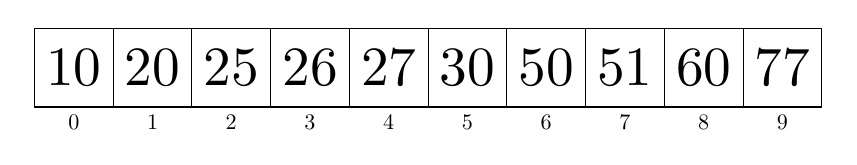
\begin{tikzpicture}
    \arraySlot{0}{three}{10}
    \arraySlot{1}{six}{20}
    \arraySlot{2}{two}{25}
    \arraySlot{3}{one}{26}
    \arraySlot{4}{four}{27}
    \arraySlot{5}{five}{30}
    \arraySlot{6}{ten}{50}
    \arraySlot{7}{eight}{51}
    \arraySlot{8}{seven}{60}
    \arraySlot{9}{nine}{77}
  \end{tikzpicture}
}
%%%%%%%%%%%%%%%%%%%%%%%%%%%%%%%%%%%
% End commands for drawing an array
%%%%%%%%%%%%%%%%%%%%%%%%%%%%%%%%%%%

% Setup listing look

\lstset{
  language=C++,
  style=eclipse,
  showspaces=false, 
  numbers=left,
  frame=tb,
}




\begin{document}
\begin{spacing}{1.1}

% Start questions
\begin{enumerate}[leftmargin=*]

% First question is the student's name
\item \textbf{Name:} \hrulefill

% A little extra space looks nice.
\vspace{.4cm}

%%%%%%%%%%%%%%%%%%%%%%%%%%%%%%%%%%%%%%%%%%%%%%%%%%%%%%%%%%%%%%%%%%%%%%%%%%%%%%%%
%%%%%%%%%%%%%%%%%%%%%%%%%%%%%%%%%%%%%%%%%%%%%%%%%%%%%%%%%%%%%%%%%%%%%%%%%%%%%%%%

\begin{lstlisting}
int f1(int n) {
  if (n == 0)
    return 1;
  else
    return n * f1(n-1);
}
\end{lstlisting}

  
\item Show the result of evaluating the function \textbf{f1} for the
  values: 0, 2, 3, 5, 7.

\vspace{4cm}

%%%%%%%%%%%%%%%%%%%%%%%%%%%%%%%%%%%%%%%%%%%%%%%%%%%%%%%%%%%%%%%%%%%%%%%%%%%%%%%%
%%%%%%%%%%%%%%%%%%%%%%%%%%%%%%%%%%%%%%%%%%%%%%%%%%%%%%%%%%%%%%%%%%%%%%%%%%%%%%%%

\begin{lstlisting}
int f2(int n) {
  if (n == 0)
    return 0;
  else if (n == 1)
    return 1;
  else
    return f2(n-1) + f2(n-2);
}
\end{lstlisting}

\item Show the result of evaluating the function \textbf{f2} for the
  values: 0, 2, 3, 5, 7.

%%%%%%%%%%%%%%%%%%%%%%%%%%%%%%%%%%%%%%%%%%%%%%%%%%%%%%%%%%%%%%%%%%%%%%%%%%%%%%%%
%%%%%%%%%%%%%%%%%%%%%%%%%%%%%%%%%%%%%%%%%%%%%%%%%%%%%%%%%%%%%%%%%%%%%%%%%%%%%%%%

\newpage

%%%%%%%%%%%%%%%%%%%%%%%%%%%%%%%%%%%%%%%%%%%%%%%%%%%%%%%%%%%%%%%%%%%%%%%%%%%%%%%%
%%%%%%%%%%%%%%%%%%%%%%%%%%%%%%%%%%%%%%%%%%%%%%%%%%%%%%%%%%%%%%%%%%%%%%%%%%%%%%%%

\begin{lstlisting}
bool f3(std::string str, int start, int end) {
  if (start >= end)
    return true;
  else
    return str[start] == str[end] && f3(str, start+1, end-1);

}
\end{lstlisting}


\item Show the result of evaluating the function \textbf{f3} for the strings:
  \lstinline$"b","be","bb","bye","bob"$. Assume that $0$ and $n-1$ are
  initially passed to the function and that $n$ is the length of the string.

\vspace{2cm}

%%%%%%%%%%%%%%%%%%%%%%%%%%%%%%%%%%%%%%%%%%%%%%%%%%%%%%%%%%%%%%%%%%%%%%%%%%%%%%%%
%%%%%%%%%%%%%%%%%%%%%%%%%%%%%%%%%%%%%%%%%%%%%%%%%%%%%%%%%%%%%%%%%%%%%%%%%%%%%%%%

\begin{lstlisting}
int f4(int list[], int key, int min, int max) {
  if (min > max)
    return -1;
  else {
    int mid = (min+max)/2;
    
    if (key < list[mid])
      return f4(list, key, min, mid-1);
    else if (key > list[mid])
      return f4(list, key, mid+1, max);
    else
      return mid;
  }
}
\end{lstlisting}

\item Show the result of evaluating the function \textbf{f4} on the array shown
  below for key values 25, 77, 10, 30, 9.  Assume that min is 0 and max
  is 9 for the initial function call.

\displayArray 

\vspace{2.5cm}

%%%%%%%%%%%%%%%%%%%%%%%%%%%%%%%%%%%%%%%%%%%%%%%%%%%%%%%%%%%%%%%%%%%%%%%%%%%%%%%%
%%%%%%%%%%%%%%%%%%%%%%%%%%%%%%%%%%%%%%%%%%%%%%%%%%%%%%%%%%%%%%%%%%%%%%%%%%%%%%%%

% !!!Important!!! Label the last item as the last question so it will
% automatically tally correctly
\item\label{lastQuestion} For each function, indicate the base cases
  and the recursive cases.  Are there any preconditions that must be
  satisfied in order for the functions to work correctly?  List the
  functions by efficiency (worst case) below.


%%%%%%%%%%%%%%%%%%%%%%%%%%%%%%%%%%%%%%%%%%%%%%%%%%%%%%%%%%%%%%%%%%%%%%%%%%%%%%%%
%%%%%%%%%%%%%%%%%%%%%%%%%%%%%%%%%%%%%%%%%%%%%%%%%%%%%%%%%%%%%%%%%%%%%%%%%%%%%%%%


\end{enumerate}
\end{spacing}

\end{document}


